\chapter{Statistics}\label{chapter:stats}

This chapter provides an overview of the statistics used
in LingPipe as well as the statistical utilities provided
as classes and methods by LingPIpe.  

\section{Useful Functions}


\subsection{The Factorial Function}\label{section:stats-factorial}

The factorial function computes the number of different ordered
permutations there are of a list of a given (non-negative) number of
distinct objects.  The factorial function is written $n!$
and defined for $n \in \nats$ by
%
\begin{equation}
n! = 1 \times 2 \times \cdots \times n = \prod_{m=1}^n m.
\end{equation}
%
The convention is to set $0! = 1$ so that the boundary conditions of
definitions like the one we provided for the binomial coefficient work
out properly.


\subsection{Binomial Coefficients}\label{section:stats-binomial-coefficient}

The binomial coefficient has many uses.  We're mainly interested in
combinatorics, so we think of it as providing the number of ways to
select a subset of a given size from a superset of a given size.  The
binomial coefficient is written ${m choose n}$, prounced ``$m$
choose $n$,'' and defined for $m, n \in \nats$ with $n \geq m$ by
%
\begin{equation}
{n \choose m} = \frac{n!}{m! \ (n-m)!}.
\end{equation}


\subsection{The $\Gamma$ Function}\label{section:stats-gamma-function}

The $\Gamma$ function is the complex generalization of the factorial
function (see \refsec{stats-factorial}).  It is written $\Gamma(x)$, 
and we're only concerned with real $x \in [0,\infty)$, where its value
is defined by 
%
\begin{equation}
\Gamma(x) = \int_0^{\infty} t^{x-1} \ \exp(-t) \ dt.
\end{equation}
%
In general, we have
%
\begin{equation}
\Gamma(x+1) = x \times \Gamma(x).
\end{equation}
%
Because $\Gamma(1) = 1$, for all $n \in \nats, n > 0$, we also have
%
\begin{equation}
\Gamma(n) = (n-1)!.
\end{equation}


\section{Discrete Probability Distributions}


\subsection{Binomial Distribution}

\subsubsection{Distribution}

The binomial distribution is parameterized by a chance-of-success
parameter $\theta \in [0,1]$ and a number-of-trials parameter $N \in
\nats$.  If a random variable $X$ has a binomial distribution with
parameters $\theta$ and $N$, we write $X \sim \dbin{\theta}{N}$.  The
probability distribution for $X \sim \dbin{\theta}{N}$ is given by 
%
\begin{equation}
p_X(n) = {N \choose n} \ \theta^{n} \ (1-\theta)^{N-n}.
\end{equation}
%
%

\subsubsection{Variance}\label{section:stats-binomial-variance}

The variance and standard deviation of a binomially-distributed random
variable $X \sim \dbin{\theta}{N}$ are given by
%
\begin{equation}
\hfill
\var{X} = \frac{\theta (1 - \theta)}{N} 
\hspace*{0.25in}
\mbox{and}
\hspace*{0.25in}
\sd{X} = \sqrt{\frac{\theta (1 - \theta)}{N}}.
\hfill
\end{equation}
%

We are often more interested in the percentage of the $N$ trials that
resulted in success, which is given by the random variable $X/N$ (note
that $N$ is a constant here).  The variable $X/N$ is scaled to be
between 0 and 1.  With large $N$, $X/N$, will be approximately equal
to $\theta$ for almost every trial.  The variance and standard
deviation of $X/N$ are derived in the usual way, by dividing by the
constant $N$,
%
\begin{equation}
\var{X/N} = \theta (1 - \theta) 
\hspace*{0.25in}
\mbox{and}
\hspace*{0.25in}
\sd{X/N} = \sqrt{\theta (1-\theta)}.
\end{equation}


\subsection{Normal Distribution}\label{section:stats-normal-distribution}



\subsection{$\chi^2$ Distribution}\label{section:stats-chi-squared-distribution}

The $\chi^2$ distribution with $n$ degrees of freedom arises as the
sum of the squares of $n$ independent unit normal distributions (see
\refsec{stats-normal-distribution}).  In symbols, if $X_n \sim \dnorm(0,1)$
for $n \in 1{:}N$, then 
%
\begin{equation}
Y = \sum_{n=1}^N X_n^2
\end{equation}
%
has a $\chi^2$ distribution with $N$ degrees of freedom.

If a variable $X$ has a $\chi^2$ distribution with $N$ degrees of
freedom, we write $X \sim \dchisq{N}$.  The probability distribution
for $X$ is defined for $x \in [0,\infty)$ by
%
\begin{equation}
p_X(x) = \frac{1}{2^{N/2} \ \Gamma(n/2)} \ x^{N/2-1} \ \exp(-x/2).
\end{equation}
%

If $X \sim \dchisq{N}$, then the mean of $X$ is
%
\begin{equation}
\expect{X} = N.
\end{equation}
%
The variance and standard deviation are equally simple, being
%
\begin{equation}
\var{X} = 2n \ \ \ \ \mbox{and} \ \ \ \  \sd{X} = \sqrt{2n}.
\end{equation}



\section{Information Theory}

\subsection{Entropy}\label{section:stats-entropy}

Entropy is an information-theoretic measure of the randomness of a
distribution.  

\subsubsection{Entropy of a Discrete Random Variable}

Suppose we have a discrete random variable $X$ taking
on values in $\nats$.  The entropy of $X$, $\entropy{X}$, is defined by
%
\begin{equation}
\entropy{X} = - \sum_{n \in \nats} p_X(n) \ \log_2 p_X(n).
\end{equation}
%
Because we use base 2 for the logs, the units are bits.  

For example, if we have a Bernoulli-distributed random
variable $Y \sim \dbern{\theta}$, its entropy is
%
\begin{align}
\entropy{Y} &= - p_Y(1) \log_2 p_Y(1) - p_Y(0) \log_2 p_Y(0)
\\
&= - \theta \log_2 \theta - (1 - \theta) \log_2 (1 - \theta).
\end{align}
%
A plot of $\entropy{Y}$ for $Y \sim \dbern{\theta}$ is provided
in \reffig{bern-entropy}.
%
\begin{figure}
\begin{center}
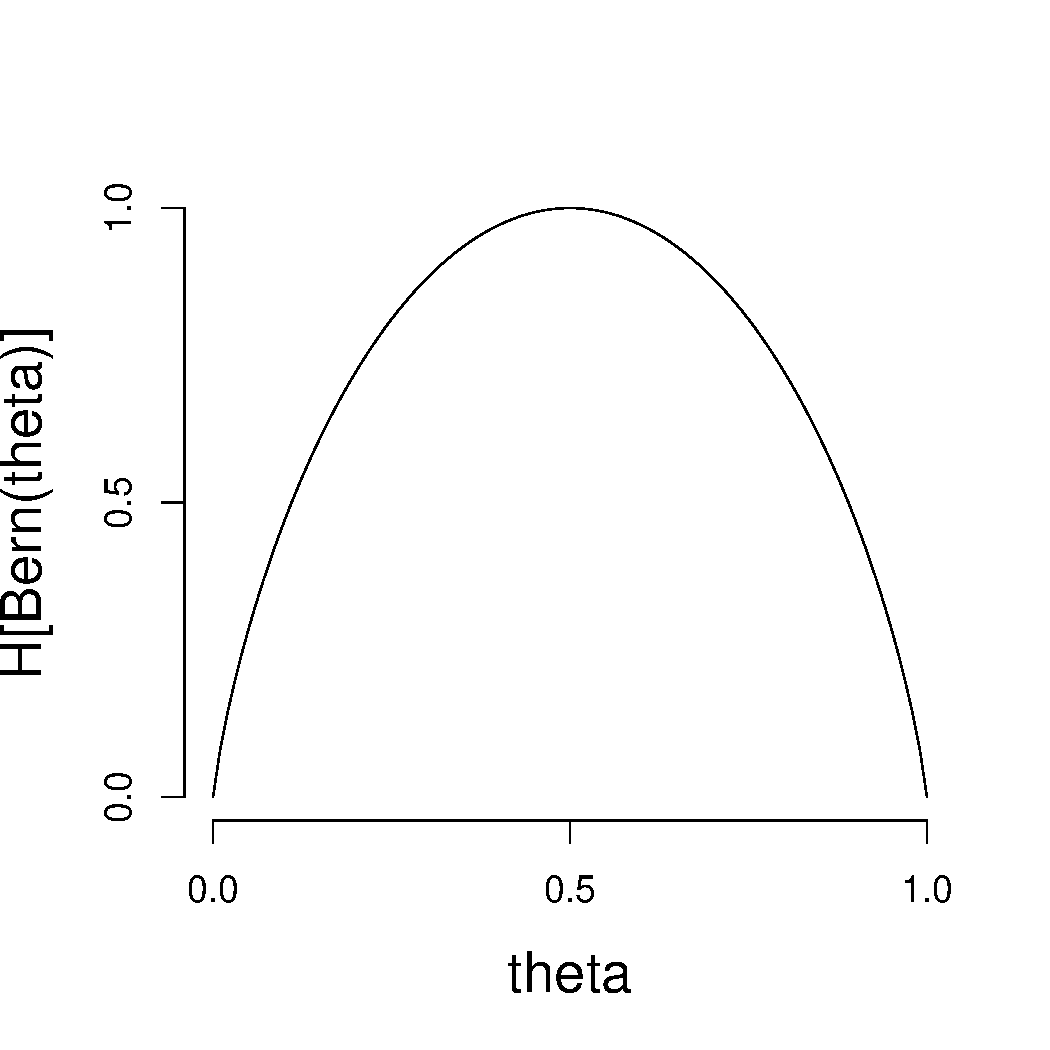
\includegraphics[height=1.75in]{pdfs/bern-entropy.pdf}
\end{center}%
\vspace*{-18pt}
\caption{Entropy of a random variable distributed as $\dbern{\theta}$.}\label{fig:bern-entropy}
\end{figure}
%
The graph makes it clear that when $\theta=0$ or $\theta=1$, the
outcome is certain, and therefore the entropy is 0.  The maximum
entropy possible for a Bernoulli distribution is 1 bit, achieved at
$\theta = 0.5$.  

\subsubsection{Entropy of a Continuous Random Variable}

As usual, to move to the continous domain, we replace our summations
with integrals and proceed as usual.  For entropy, suppose we
have a continuous random variable $X$ taking on values in $\reals$.
The entropy of $X$, also written as for the discrete case as $\entropy{X}$,
is defined by
%
\begin{equation}
\entropy{X} = - \int_{-\infty}^{\infty} p_X(x) \ \log_2 p_X(x) \ dx
\end{equation}


\subsubsection{Entropy as an Expectation}

Entropy may also be expressed, in both the discrete and continous cases,
as the expectation of the negative log probability.  Specifically, we have
%
\begin{equation}
\entropy{X} = \expect{- \log_2 p_X(X)}.
\end{equation}


\subsubsection{Entropy and Compression}

Entropy has a natural interpretation in terms of compression.  Suppose
we want to send the a message $X$ which might take on values in
$\nats$.%
%
\footnote{We can always code sequences of characters as numbers, as
originally noted by Kurt G\"odel, and as explained in any introductory
computer science theory text.  Just think of a string as representing
a number in the base of the number characters.}
%
If the sender and receiver both know the distribution $p_X$
of outcomes, the expected cost to send the message is $\entropy{X}$
bits.  For instance, if we need to send a bit with value 0 or 1, and
each outcome is equally likely, it will require 1 bit to send the
message.  On the other hand, if one outcome is more likely than the
other, we can save space (if we have repeated messages to send;
otherwise, we must round up).

\subsubsection{Joint Entropy}\label{section:stats-joint-entropy}

We can measure the entropy of two variables $X$ and $Y$ by measuring
the entropy of their joint distribution $p_{X,Y}$, generalizing our definition
to
%
\begin{equation}
\entropy{X,Y} = - \sum_{x,y} p_{X,Y}(x,y) \ \log_2 p_{X,Y}(x,y).
\end{equation}
%
This is just what we'd get by computing the entropy of the outcomes
of the multivariate random variable $Z = (X,Y)$.

\subsubsection{Conditional Entropy}\label{section:stats-conditional-entropy}

We can measure the entropy of a variable $X$ conditional on knowing
the value of another variable $Y$.  We do this by measuring the
entropy of the conditional distribution $p_{X|Y}$, weighting
over the marginal distribution $p_Y$, giving us
%
\begin{equation}
\condentropy{X}{Y} = - \sum_y p_Y(y) \sum_x p_{X|Y}(x|y) \ \log_2 p_{X|Y}(x|y).
\end{equation}
%

Conditional entropy, joint entropy and entropy are related as for
probabilty distributions, with
%
\begin{equation}
\condentropy{X}{Y} = \entropy{X,Y} - \entropy{Y}.
\end{equation}


\subsubsection{Mutual Information}\label{section:stats-mutual-information}

The mutual information between a pair of variables $X$ and $Y$ measures how
much more information there is in knowing their joint distribution than their
individual distributions for prediction.  The definition for the discrete case is
%
\begin{equation}
\mutualinfo{X}{Y} = \sum_{x,y} p_{X,Y}(x,y) \ \log_2 \frac{p_{X,Y}(x,y)}{p_X(x) \ p_Y(y)}.
\end{equation}
%
As with the other definitions, it may be expressed as an expectation, with
%
\begin{equation}
\mutualinfo{X}{Y} = \expect{\log_2 \frac{p_{X,Y}(x,y)}{p_X(x) \ p_Y(y)}}
\end{equation}

Mutual inforamtion is symmetric.  It's related to conditional and joint entropies by
%
\begin{align}
\mutualinfo{X}{Y} &= \entropy{X} + \entropy{Y} - \entropy{X,Y}
\\
&= \entropy{X} - \condentropy{X}{Y}.
\end{align}
%


\subsection{Divergence}\label{section:stats-divergence}

Kullback-Leibler (KL) divergence is the standard method to compare the
distributions of two random variables.  Pairs of topic distributions
that have similar probability assignments to words will have low KL
divergences from each other.

We will start with the discrete case, as it is what Griffiths and
Steyvers used in their experiments.  We'll consider the continuous
case, and specifically consider the Dirichlet distributions underlying
the LDA models.

\subsubsection{Cross Entropy}\label{section:stats-cross-entropy}

Cross entropy measures the ability of one distribution to represent
results drawn from another distribution.  Given two discrete random
variables $X$ and $Y$ with outcomes ranging from 1 to $N$, we define
the cross entropy of $X$ with respect to $Y$ as
%
\begin{equation}
\xentropy{X}{Y} = \sum_{n=1}^N p_X(n) \ \log_2 p_Y(n).
\end{equation}
%
This value measures the number of bits required, on average, to
transmit a value of $X$ using the distribution of $Y$ for coding.


\subsubsection{Defining KL Divergence}

As is standard, our definition will use random variables, but we point
out ahead of time that only the distributions of the variables matter,
not the outcomes.  Suppose that $X$ and $Y$ are two random variables
with possible outcomes ranging from 1 to $N$ and probabilty
distributions $p_X(n)$ and $p_Y(n)$.  The KL divergence of $X$ from
$Y$ is given by
%
\begin{equation}
\kld{X}{Y}
= \sum_{n=1}^N p_X(n) \log_2 \frac{p_X(n)}{p_Y(n)}.
\end{equation}
%
Because we used base-2 logs, the result is in units of bits.  Note
that this value is just the entropy of $X$ minus the cross entropy
of $X$ with respect to $Y$

If there is an outcome $n$ where $p_Y(n) = 0$ and $p_X(n) > 0$, the
divergence is infinite.  We may allow $p_X(n) = 0$ by interpreting $0
\log_2 \frac{0}{p_Y(n)} = 0$ by convention (even if $p_Y(n) > 0$).

Although we do not provide a proof, we note that $\kld{X}{Y} \geq 0$
for all random variables $X$ and $Y$.  We further note without proof
that $\kld{X}{Y} = 0$ if and only if $p_X = p_Y$.

For example, suppose we have three discrete random variables, $X$, $Y$
and $Z$, each with the same two outcomes, and distributions defined by
$p_X(1) = 0.2$, $p_X(2) = 0.8$ and $p_Y(1) = 0.4$, $p_Y(2) = 0.6$.  We
calculate 
%
\[
\kld{X}{Y} = 0.2 \log_2 (0.2/0.4) + 0.8 \log_2 (0.8/0.6) \approx 0.13.
\]
%
Consider a third random variable, $Z$, with $p_Z(1) = 0.5$ and
$p_Z(2) = 0.5$.  The KL-divergence calculation is 
%
\[
\kld{X}{Z} = 0.2 \log_2 (0.2/0.5) + 0.8 \log_2 (0.8/0.5) \approx 0.27.
\]
As we'd expect, $Z$ diverges further from $X$ than $Y$.  
Comparing $X$ to itself, we get
%
\[
\kld{X}{X} = 0.2 \log_2 (0.2/0.2) + 0.8 \log_2(0.8/0.8) = 0.
\]  
%
From this example, it's easy to see why $\kld{X}{X}$ is always 0.

KL divergence may expressed using expectation notation as
%
\begin{align}
\kld{X}{Y} 
&= \expect{\log_2 \frac{p_X(X)}{p_Y(X)}}
\\
&= \expect{\log_2 p_X(X)} - \expect{\log_2 p_Y(X)}.
\end{align}
%
As usual, unmarked expectation notation presupposes the natural
distributions for random variables, here using the distribution $p_X$
for the random variable $X$.%
%
\footnote{The first term is just the entropy of $X$,
$\entropy{X} = \expect{\log_2 p_X(X)}$.  Another way of interpreting
KL divergence is as the expected penalty in bits for using $p_Y$ to
model values of $X$ rather than $p_X$.}

\subsubsection{Symmetrized KL Divergence}\label{section:stats-symmetrized-kl-divergence}

KL divergence is not symmetric in the sense that there exist pairs of
random variables $X$ and $Y$ such that $\kld{X}{Y} \neq \kld{Y}{X}$.
We have an example to hand.  Consider our example $X$ and $Y$ above,
for which we noted $\kld{X}{Y} \approx 0.13$.  The other way around,
$\kld{Y}{X} = 0.4 \log_2 0.4/0.2 + 0.6 \log_2 0.6/0.8 \approx 0.15$.

There are several divergence measures derived from KL divergence that
are symmetric.  The simplest approach is just to introduce symmetry
by brute force.  The symmetrized KL-divergence between random variables
$X$ and $Y$ is defined by averaging KL divergence of $X$ from $Y$
and of $Y$ from $X$,
%
\begin{equation}
\skld{X}{Y} = \frac{1}{2}(\kld{X}{Y} + \kld{Y}{X}).
\end{equation}
%
Obviously, $\skld{X}{Y} = \skld{Y}{X}$, so the measure is symmetric.


\subsubsection{Jensen-Shannon Divergence}

Another widely used symmetric divergence measure derived from KL divergence
is the Jensen-Shannon divergence.  To compare $X$ and $Y$ using Jensen-Shannon
divergence, we first define a new random variable $Z$ with distribution defined by
averaging the distributions of $X$ and $Y$,
%
\[
p_Z(n) = \frac{1}{2}(p_X(n) + p_Y(n)).
\]
%
We then define Jensen-Shannon divergence by taking average divergence
from $Z$,
%
\begin{equation}
\jsd{X}{Y} = \frac{1}{2}(\kld{X}{Z} + \kld{Y}{Z}).
\end{equation}
%
As with the symmetrized KL divergence, Jensen-Shannon divergence is
symmetric by definition.


\subsubsection{LingPipe KL-Divergence Utilities}

KL-divergence is implemented as a static utility method in the
\code{Statistics} utility class in package \code{com.aliasi.stats}.
The method takes two double arrays representing probability
distributions and measures how much the first is like the second.

In order to give you a sense of KL-divergence, we implement a simple
utility in the demo class \code{KlDivergence} to let you try various
values.  The code just parses out double arrays from teh command line
and sends them to the KL function.
%
\codeblock{KlDivergence.1}

The ant target \code{kl} runs the command with the first two arguments
given by properties \code{p.x} and \code{p.y}.  To calculate the example
from above, we have
%
\commandlinefollow{ant -Dp.x="0.2 0.8" -Dp.y="0.4 0.6" kl}
\begin{verbatim}
pX=(0.2, 0.8)     pY=(0.4, 0.6)     
kld=0.13202999942307514    
skld=0.1415037499278844   
jsd=0.03485155455967723
\end{verbatim}
%
The Jensen-Shannon divergence is less than the symmetrized KL
divergence because the interpolated distribution $p_Z$ is closer to
both of the original distributions $p_X$ and $p_Y$ than they are to
each other.

